\documentclass{subfiles}

\begin{document}
    \marginnote{\textbf{\textit{VL 6}}\\20.04.2023, 10:00}[-1cm]
    \paragraph*{Aufbau von Atomen, Isotopie}
        Zusammenfassend haben wir festgestellt, daß Atome aus Elektronen ($e^-$) in der Hülle und Protonen ($p^+$) im Kern bestehen müssen. Noch nicht erwähnt sind die sogenannten \href{https://de.wikipedia.org/wiki/Neutron}{\emph{Neutronen}} ($n^0$), welche sich ebenfalls im Kern ansiedeln. Wir definieren nun den Begriff \emph{Isotop}, welcher ein Atom (also Element) beschreibt, bei welchem sich die Anzahl der Neutronen ändert, jedoch die Protonenanzahl gleich bleibt. Beipiel ist der Wasserstoff (H), welcher sich in \emph{Protium} ($^1_1\text{H}$), \emph{Deuterium} ($^2_1\text{H}$) und \emph{Tritium} ($^3_1\text{H}$) unterteilt, bei welchen die letzten beiden Isotope natürlich eher selten anzutreffen sind. 

    \subsection{Entwicklung der Quantenmechanik}
        Wichtige Experimente waren
        \begin{itemize}
            \item Das \href{https://de.wikipedia.org/wiki/Doppelspaltexperiment}{\emph{Doppelspaltexperiment}} von \href{https://de.wikipedia.org/wiki/Thomas_Young}{Thomas Young} (1801), welches den Welle-Teilchen-Dualismus fundierte.
            \item Die \href{https://de.wikipedia.org/wiki/Schwarzer_Körper}{\emph{Schwarzkörperstrahlung}} von \href{https://de.wikipedia.org/wiki/Max_Planck}{Max Planck} (1900), welche die Quantisierung der Strahlung beschrieb.
            \item Der \href{https://de.wikipedia.org/wiki/Photoelektrischer_Effekt}{\emph{photoelektrische Effekt}} von \href{https://de.wikipedia.org/wiki/Albert_Einstein}{Albert Einstein} (1905), welcher die Quantisierung der Photonen beschrieb.
            \item Der \href{https://de.wikipedia.org/wiki/Compton-Effekt}{\emph{Compton-Effekt}} von \href{https://de.wikipedia.org/wiki/Compton-Effekt}{Compton-Effekt} (1923), welcher die Lichtstreuung an freien Elektronen beschrieb (Welle-Teilchen-Dualismus).
            \item Die \href{https://de.wikipedia.org/wiki/De_Broglie-Wellenl%C3%A4nge}{\emph{De Broglie-Wellenlänge}} von \href{https://de.wikipedia.org/wiki/Louis_de_Broglie}{Louis de Broglie} (1924), welche die Wellenlänge von Teilchen/Materie beschrieb.
            \item Die \href{https://de.wikipedia.org/wiki/Spektrallinie}{\emph{Spektrallinien}} von \href{https://de.wikipedia.org/wiki/Johann_Jakob_Balmer}{J. Balmer} (1885), welche die Quantisierung der Atomenergie durch Absorbtion und Emission von Licht beschrieb. Dies führte zur Entwicklung des Atommodells durch \href{https://de.wikipedia.org/wiki/Niels_Bohr}{Niels Bohr} (1913).
        \end{itemize}

        \subsubsection{Schwarzkörperstrahlung}
            \paragraph*{Der schwarze Körper / Hohlraumstrahlung}

                Interessant ist die quantitative Beschreibung dieser Phänomene, z.B. durch die Intensitätsverteilung im Spektrum eines Körpers. 

                Der \emph{schwarze Körper} ist ein Körper mit einer Oberfläche, welche alle Strahlung absorbiert, d.h. der Absorbtionskoeffizient des Körpers ist $A=1$, woraus mit $A+R=1$ wiederum folgt $R=0$ für alle $\lambda\in\R$. Somit muss ein Körper, welcher alle Strahlung absorbiert, auch alle Strahlung emittieren, und dies proportional zu seiner Temperatur. Dies ist die Grundlage des \emph{Planckschen Strahlungsgesetz}. Anschaulich passiert mit einfallender Strahlung auf einen Schwarzkörper folgendes:
                \begin{figure}
                    \centering
                    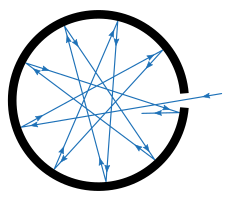
\includegraphics[width=5cm]{Bilddateien/Black_body_realization.svg.png}
                    \caption{Schema eines Schwarzkörpers \cite{wiki:BlackBody}.}
                    \label{fig:SchwarzkoerperSchema}
                \end{figure}
                Die Intensitätsverteilung der austretenden Strahlung ist identisch mit derjenigen des sich im Hohlraum befindlichen EM-Felder. Das spektrale Emissionsvermögen eines schwarzen Körpers ist also identisch mit der spektralen Strahlungsdichte der Hohlraumstrahlung. 

                \begin{Aufgabe}
                    \nr{} Recherchiere die \href{https://de.wikipedia.org/wiki/Dyson-Sphäre}{\emph{Dyson-Sphäre}}. Handelt es sich um einen Schwarzkörper?
                \end{Aufgabe}

                \begin{Experiment}{Die Glühbirne}
                    Wir starten bei $6\si\watt$. Das Licht einer Glühbirne wird spektral zerlegt. Ein Detektor misst die Strahlungsintensität und abhängig von der Wellenlänge. Wir sehen einen Peak und Maximum im Ifraroten Bereich. Dies ist die \href{https://de.wikipedia.org/wiki/Infrarotstrahlung}{\emph{Infrarotstrahlung}} der Glühbirne.\\
                    
                    Nun ändern wir die Leistung auf $3\si\watt$; sofort wird das sichtbare Spektrum schwächer auf dem Schirm abgebildet. Die erhaltene Intensitätskurve ist relativ zu der $6\si\watt$ Kurve nach oben verschoben. Wir sehen, daß der Peak (nach rechts, ins Infrarote) verschoben ist. (Das Experiment wurde aufgrund zu flacher Kurve hier abgebrochen.)

                    Hinweis: Simuliere das Experiment auf der \href{https://tetfolio.fu-berlin.de/web/1089581}{FU-Berlin} Website.
                \end{Experiment}

                \noindent Aus klassischer Sicht ergibt sich für die spektrale Energiedichte 
                \[u(\nu,T)\cdot d\nu = \frac{8\cdot\pi}{c^3}\cdot\nu^2\cdot k_B\cdot T\cdot d\nu,\]
                auch bekannt als \href{https://de.wikipedia.org/wiki/Rayleigh-Jeans-Gesetz}{\emph{Rayleigh-Jeans-Gesetz}}. Für $\nu\to\infty$ erfolgt eine sogenannte \emph{Ultraviolettkatastrophe}. Dieses Verhalten ist jedoch nur bei klassischer Strahlung zu beobachten. Das Modell weist eine gute Übereinstimmung mit der Realität für kleine Frequenzen auf.

                \begin{Aufgabe}
                    \nr{} Recherchiere den \href{https://de.wikipedia.org/wiki/Gleichverteilungssatz}{\emph{Gleichverteilungssatz}}. Wie fließt er in das Rayleigh-Jeans-Gesetz ein?
                \end{Aufgabe}

            \paragraph*{Plancksches Strahlungsgesetz}
                Max Planck leitete die korrekte Strahlungsformel für das beobachtete Phänomen und Diskrepanz her. Wir konzentrieren uns nachfolgend jedoch auf die Herleitung nach Einstein. \\

                \noindent\underline{Annahmen.} Wir müssen annehmen, daß Licht aus Teilchen besteht, die sogenannten Photonen, und damit quantisiert ist. Weiter nehmen wir an, daß Atome diskrete Energieniveaus besitzen müssen. Es gibt insbesondere \emph{nur} zwei, welche wir $E_1$ und $E_2$ mit $E_2>E_1$ nennen wollen. \\

                Damit kommen zwei Prozesse bei der Wechselwirkung mit der elektromagnetischen Strahlung infrage: (i) Absorbtion und (ii) Reflexion. \\

                \noindent\underline{Prozess (i).} Bei der Absorbtion eines Photons mit Energie $E=E_2-E_1= h\cdot\nu$ wird das Atom von $E_1$ auf $E_2$ angeregt\footnote{Es ist $h=6.62\cdot 10^{-34}\si{\joule\second}$ die \href{https://de.wikipedia.org/wiki/Planck-Konstante}{\emph{Planck-Konstante}} und $\hbar:=h/(2\cdot\pi)$ die reduzierte Variante.}.

                \noindent\underline{Prozess (ii).} Im angeregten Zustand kann das Atom \emph{spontan} das Energieminimm anstreben und ein Photon der Energie $E_2-E_1=h\cdot\nu$ emittieren. \\

                Anschaulich sind die Prozesse wiefolgt, wobei noch die \emph{induzierte Emission} als Kombination beigefügt wurde:
                \begin{figure}
                    \centering
                    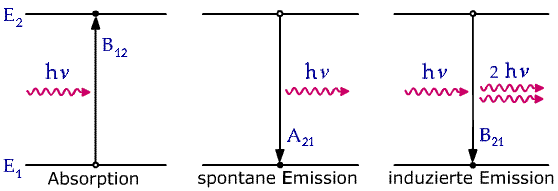
\includegraphics[width=5cm]{Bilddateien/AtomPhotonEmission.gif}
                    \caption[short]{Schema der Emission eines Photons durch eine Atomanregung \cite{uniulm:PlanckStrahlung}.}
                \end{figure}
                In einem Atomsystem mit $N\in\N$ Atomen haben wir $N_1$ Atome in Zustand $E_1$ und $N_2$ Atome in Zustand $E_2$. Für die Prozesse gilt dann:\\

                \noindent\underline{Prozess (i).} Für ein Atom in Zstand $E_1$ gilt die Änderung 
                \[dN_{12} =\lint{B_{12}\cdot u(\nu,T)\cdot N_1}{t}{},\]
                wobei $B_{12}$ ein \emph{Einstein Koeffizient} ist, welcher die Übergangswahrscheinlichkeit angibt in der Einheit $[1/(s\cdot J/m^3)]$ mit $E$ als Energiedichteeinheit. 

                \noindent\underline{Prozess (ii).} Für ein Atom in Zustand $E_2$ gilt die Änderung
                \[dN_{21} = \lint{A_{21}\cdot N_2}{t}{},\]
                mit $A_{21}$ als \emph{Einstein Koeffizient}. 


\end{document}